\documentclass{article}
\usepackage{pgf,tikz,tikzscale} 
\usepackage{amssymb}
\usepackage{tcolorbox}
\usepackage{xcolor}
\usepackage[utf8]{inputenc}
\usepackage[english]{babel}
\usepackage{multicol}
\usepackage{enumerate}	
\usepackage{graphicx,lipsum,pgfplots} 
\usepackage{amsmath, amsthm}                 
\usepackage[top=1in,bottom=1in, left=1in, right=1in] {geometry}  
\usepackage{fancyhdr}       
\usepackage{blkarray}


\pagestyle{fancy}              
\lhead{Math 5563 \newline Graph Theory HW2, Ch1}   
\rhead{Warren Keil}







\begin{document}
\setlength{\parindent}{0cm}   %%%%%%%% KEEP THIS  for block style paragraphs. 



%%%%%%%%%%%%%%%%%        1a   %%%%%%%%%%%%%%%%%%%%
\textbf{1a.} The Hawaiian alphabet consists of the vowels a,e,i,o,u and the consonants h,k,l,m,n,p, and w. Show that 20,736 different four-letter "words" can be constructed from the 12-letter Hawaiian alphabet. 
\vspace{2mm}

\textit{Solution.} Since we are not requiring that the words are actual words in any dictionary, we simply have can use a counting argument to solve this. We have twelve choices of letter for each of the four letters. Thus the number of different words is \(4^{12} = 20736\). 

\vspace{3mm}

\textbf{1c.} How many four-letter words can be constructed from the Hawaiian alphabet if the first and third letters are consonants and the second and last letters are vowels?

\vspace{2mm}


\textit{Solution.} Again, using a counting argument, we have seven choices for the first and third letters and five choices for the second and forth letters. Thus we have 
\[
7\cdot4\cdot7\cdot4\cdot = 784 \text{ words. } 
\]

\vspace{4mm}

\textbf{2a.} Illustrate 6 different red white and blue colorings of \(K_3\). 


\vspace{2mm}

\textit{Solution.} 

\vspace{2mm}

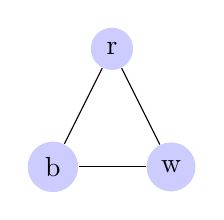
\begin{tikzpicture}
  [scale=.15,auto=left,every node/.style={circle,fill=blue!20}]
  \node (a) at (0,0) {b};
  \node (b) at (5,10)  {r};
  \node (c) at (10,0)  {w};

  \foreach \from/\to in {a/b,a/c,b/c}
    \draw (\from) -- (\to);

\end{tikzpicture} \hspace{4mm}
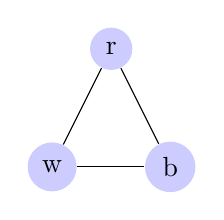
\begin{tikzpicture}
  [scale=.15,auto=left,every node/.style={circle,fill=blue!20}]
  \node (a) at (0,0) {w};
  \node (b) at (5,10)  {r};
  \node (c) at (10,0)  {b};

  \foreach \from/\to in {a/b,a/c,b/c}
    \draw (\from) -- (\to);

\end{tikzpicture}\hspace{4mm}
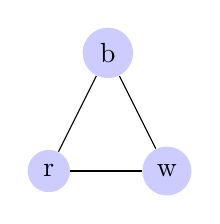
\begin{tikzpicture}
  [scale=.15,auto=left,every node/.style={circle,fill=blue!20}]
  \node (a) at (0,0) {r};
  \node (b) at (5,10)  {b};
  \node (c) at (10,0)  {w};

  \foreach \from/\to in {a/b,a/c,b/c}
    \draw (\from) -- (\to);

\end{tikzpicture}\hspace{4mm}
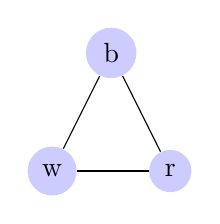
\begin{tikzpicture}
  [scale=.15,auto=left,every node/.style={circle,fill=blue!20}]
  \node (a) at (0,0) {w};
  \node (b) at (5,10)  {b};
  \node (c) at (10,0)  {r};

  \foreach \from/\to in {a/b,a/c,b/c}
    \draw (\from) -- (\to);

\end{tikzpicture}\hspace{4mm}
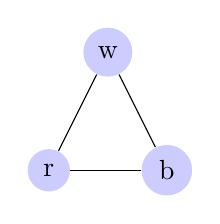
\begin{tikzpicture}
  [scale=.15,auto=left,every node/.style={circle,fill=blue!20}]
  \node (a) at (0,0) {r};
  \node (b) at (5,10)  {w};
  \node (c) at (10,0)  {b};

  \foreach \from/\to in {a/b,a/c,b/c}
    \draw (\from) -- (\to);

\end{tikzpicture}\hspace{4mm}
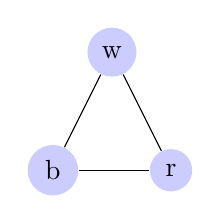
\begin{tikzpicture}
  [scale=.15,auto=left,every node/.style={circle,fill=blue!20}]
  \node (a) at (0,0) {b};
  \node (b) at (5,10)  {w};
  \node (c) at (10,0)  {r};

  \foreach \from/\to in {a/b,a/c,b/c}
    \draw (\from) -- (\to);

\end{tikzpicture}
\vspace{4mm}

\textbf{3a.} Illustrate \(G= K_2 \vee K^c_3\)


\vspace{2mm}

\textit{Solution.}


\begin{center}
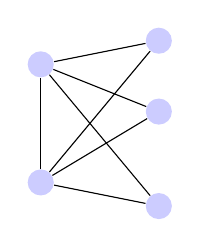
\begin{tikzpicture}
  [scale=.15,auto=left,every node/.style={circle,fill=blue!20}]
  \node (a) at (0,0) {};
  \node (b) at (0,10)  {};
  \node (c) at (10,-2)  {};
  \node (e) at (10,6)  {};
  \node (f) at (10,12)  {};


  \foreach \from/\to in {a/b,a/c,b/c,a/e,a/f,b/e,b/f}
    \draw (\from) -- (\to);

\end{tikzpicture}
\end{center}

\vspace{4mm}

\textbf{5} Prove that \(\omega\) and \(\alpha\) are graph invariants. 


\vspace{2mm}

\textit{Proof that \(\omega\) is invariant.} Let \(G= (V,E)\) and \(H=(V',E')\) be graphs such that \(G \cong H\). Let \(f:V\rightarrow V'\) be an isomorphism. Suppose \(\omega(G) = n\). Then this means that the largest clique in \(G\) has \(n\) vertices. Let \(C=\{v_1, v_2,\cdots, v_n\}\) be the set of vertices for a largest clique in \(G\). (We say \textit{a} largest clique to imply that there could be multiple largest cliques. WLOG, proving for one still proves the theorem for all). By the definition of a clique, these vertices are all pairwise connected and isomorphic to \(K_n\). Then let \(C'=\{f(v_1), f(v_2), \cdots, f(v_n)\}  \) be the set \(\{f(v) : v\in C\}\). Since every \(v\in C\) is pairwise adjacent to every other vertex in \(C\), and since \(f\) is an isomorphism from \(G\) to \(H\) then it follows that every vertex in \(C'\) must be pairwise adjacent. And since \(f\) is one to one, then \(C'\) must contain precisely \(n\) vertices. Thus, the vertices of \(C'\) form a clique in \(H\). To show that this must be a largest clique in \(H\), we will show via contradiction that there cannot be a larger clique in \(H\). So assume there exists a larger clique in \(H\). Let \(C''\) be the set of vertices in this larger clique. Then \( C'' =\{v'_1,v'_2, \cdots,v'_m\} \subseteq V' \) where \( m>n\). And since \(f\) is bijective, there exists a unique \(u \in V\) for each \(v' \in C''\). Thus we can write \(C''=\{f(u_1), \cdots f(u_m)\} \). Since each vertex in \(C'' \) is pairwise adjacent and  \(f\) is an isomorphism, then every vertex in the set \( \{ u : f(u) \in C''\}\) must also be adjacent by the properties of a graph isomorphism. Thus the set \( \{ u : f(u) \in C''\}\) is a clique in \(G\) and has \(m\) vertices \( \rightarrow\!\leftarrow \). But this contradicts our assumption that the largest clique in \(G\) had \(n\) vertices. Thus the largest clique in \(H\) must also have \(n \) vertices. Thus the clique number of \(H, \omega(H)=n\). \(\therefore \omega\) is a graph invariant. 

\begin{flushright}
\(\blacksquare\)
\end{flushright}


\newpage

\textit{Proof that \(\alpha \) is invariant}. Let \(G= (V,E)\) and \(H=(V',E')\) be graphs such that \(G \cong H\). Let \(f:V\rightarrow V'\) be an isomorphism. Suppose the independence number of \(G\),   \( \alpha(G)=n\). Then it follows that \(\omega(G^c) = n \) since by the definition of \(\alpha(G) = \omega(G^c)=n \).  And since it is trivially shown that \( G \cong H \iff G^c \cong H^c \), then we can use the fact that \( \omega(G^c)=n \iff \omega(H^c) = n \) since we proved that \( \omega \) is a graph invariant. And by the definition of independence number, \( \alpha(H) =  \omega(H^c) = n \). \(\therefore\) \( \alpha \) is a graph invariant. 

\begin{flushright}
\(\blacksquare\)
\end{flushright}


\vspace{4mm}
\textbf{14a.} Let \(T\) be a tree on \(n\) vertices, \(p\) of which are pendants. Suppose  diam\((T)=d \). Prove \(n+1 \geq p+d\). 


\vspace{2mm}

\textit{Proof.} Let \(T\) be a tree on \(n\) vertices, with \(p\) pendants. Suppose diam\((T)=d\). First remove every pendent from the graph and call this graph \(T'\). Since \(T\) is a tree, \(T'\) is also a tree but not with \(n-p\) vertices. Now it should be apparent that max distance we can have on this tree \(T'\) is if the tree contains a single branch. It follows that distance from this single branch is \( d = n-p\). Now when we add the pendents back to our tree, we observe that


\vspace{4mm}

\textbf{16a.} Illustrate a graph \(G\) where \(\chi(G)=\omega(G)\). 


\vspace{2mm}

\textit{Solution.}
\begin{center}
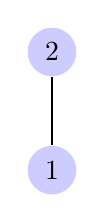
\begin{tikzpicture}
  [scale=.15,auto=left,every node/.style={circle,fill=blue!20}]
  \node (a) at (0,0) {1};
  \node (b) at (0,10)  {2};


  \foreach \from/\to in {a/b}
    \draw (\from) -- (\to);

\end{tikzpicture}
\end{center}

\vspace{4mm}

\textbf{16b.} Illustrate a graph \(G\) where \(\chi(G)=\omega(G)+1\). 


\vspace{2mm}

\textit{Solution.}
\begin{center}
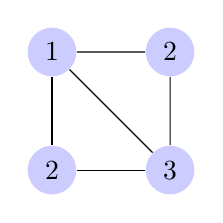
\begin{tikzpicture}
  [scale=.15,auto=left,every node/.style={circle,fill=blue!20}]
  \node (a) at (0,0) {2};
  \node (b) at (0,10)  {1};
  \node (c) at (10,0)  {3};
  \node (e) at (10,10)  {2};


  \foreach \from/\to in {a/b,a/c,b/c,c/e,b/e}
    \draw (\from) -- (\to);

\end{tikzpicture}
\end{center}


\vspace{4mm}

\textbf{16c.} Illustrate a graph \(G\) where \(\chi(G)=\omega(G)+2\). 


\vspace{2mm}

\textit{Solution.}




\vspace{40mm}


\newpage
\textbf{34.} A \textit{cotree} is a graph whose complement is a tree. Illustrate the nonisomorphic cotrees on \(n=5\) vertices. 


\vspace{2mm}

\textit{Solution.}


\vspace{60mm}

\textbf{35.} Let \(G\) be a connected graph. Prove or disprove that the diameter of \(G\) is equal to the length of a longest path in \(G\). 


\vspace{2mm}

\textit{Solution.} Disprove. Observe this counter example.











\end{document}
